%\VignetteIndexEntry{SDAMS Vignette}
%\VignettePackage{SDAMS}
%\VignetteKeyword{Semi-parametric Differential Adundance Analysis}

\documentclass[12pt]{article}

\usepackage{float}
\usepackage{Sweave}

\usepackage{amssymb}


\RequirePackage{Bioconductor}
\AtBeginDocument{\bibliographystyle{unsrturl}}

\renewcommand{\baselinestretch}{1.3}






\author{Yuntong Li$^{1}$, Chi Wang$^{2,3}$\footnote{to whom correspondence
should be addressed}, Li Chen$^{2,3}$\footnote{to whom correspondence
should be addressed}\\[1em]
\small{$^{1}$Department of Statistics , University of Kentucky,Lexington, KY;}\\
\small{$^{2}$Markey Cancer Center, University of Kentucky, Lexington, KY ;}\\
\small{$^{3}$Department of Biostatistics, University of Kentucky,
Lexington, KY;}\\
\small{\texttt{yuntong.li@uky.edu}}\\
\small{\texttt{chi.wang@uky.edu}}\\
\small{\texttt{lichenuky@uky.edu}}}



\title{\textsf{\textbf{The SDAMS package}}}

%\bibliographystyle{abbrv}

\begin{document}
\input{SDAMS-concordance}
\maketitle

\begin{abstract}
This vignette introduces the use of the Bioconductor package
{\tt SDAMS}, which is designed for differential abundance analysis for
metabolomics and proteomics data from mass spectrometry. These data may contain
a large fraction of zero values and non-zero part may not be normally
distributed. {\tt SDAMS} considers a two-part semi-parametric mdoel, a logistic
regression for the zero proportion and a semi-parametric log-linear model for
the non-zero values. A kernel-smoothed likelihood method is proposed to estimate
regression coefficients in the two-part model and a likelihood ratio test is
constructed for differential abundant analysis.

\end{abstract}


\newpage

\tableofcontents

\newpage


\section{Citation}
The package {\tt SDAMS} implements statistical methods from the following
publication. If you use {\tt SDAMS} in the published research, please cite: \\
Yuntong Li, Teresa W.M. Fan, Andrew N. Lane, Woo-Young Kang, Susanne M. Arnold,
Arnold J. Stromberg, Chi Wang and Li Chen: A Two-Part Semi-Parametric Model for
Metabolomics and Proteomics Data. (Manuscript)

\section{Quick Start}
This section show the most basic {\tt SDAMS} work flow for a differential
abundance analysis for metabolomics and proteomics data:
\begin{enumerate}
\item Create a {\tt SummarizedExperiment} object using function
      {\tt createSEsetFromEnvir} or {\tt createSEsetFromCSV}.
      In this section we use an example {\tt SummarizedExperiment} set directly,
      which is an object of {\tt SummarizedExperiment} class named
      {\tt exampleSumExpset} contained in this package.
\item Perform a differential abundance analysis using {\tt SDA}.
\end{enumerate}


\begin{Schunk}
\begin{Sinput}
> library("SDAMS")
> data("exampleSumExpset")
> results=SDA(exampleSumExpset)
\end{Sinput}
\end{Schunk}

Here, the {\tt SummarizedExperiment} class {\tt exampleSumExpset} contained in
the package is the proteomics dataset, which a matrix-like container for
proteomics features with experimental subject grouping information. There are
560 features for 202 experimental subjects (0 for control and 1 for patient).
This is a 10\% subsample of the original dataset. Each row in this matrix
repressents a proteomics feature. See Reference~ \cite{siwy2011human} for
detailed information regarding this dataset.



\section{Data Input}


\subsection{Create SummarizedExperiment object from csv.files}
The proteomics or metabolomics data is stroed as a matrix with each
row being a feature and each column corresponding to a subject. All data in this
matrix are non-negative. Another information required is the phenotype
covariates. Here we focus on the binary grouping information, such as numeric 1
for control group and 0 for case group. But it can also be characters, such as
"healthy" and "disease". To utlize {\tt SDAMS} package, we should have two
separate csv.files (for example 'feature.csv' and 'group.csv') as inputs for
{\tt createSEsetfromCSV} to creat a {\tt SummarizedExperiment} object.

Note:
\begin{enumerate}
\item The $1^{st}$ column in 'feature.csv' represents feature names and the
      $1^{st}$ row represents subject codes.
\item The $1^{st}$ column in 'group.csv' represents subject codes, for example,
      Subject1, Subject2....
\end{enumerate}


The format for "csv.files" should looks like as Figure~\ref{example feature}
and Figure~\ref{example group}:

\begin{figure}[h!]
  \centering
  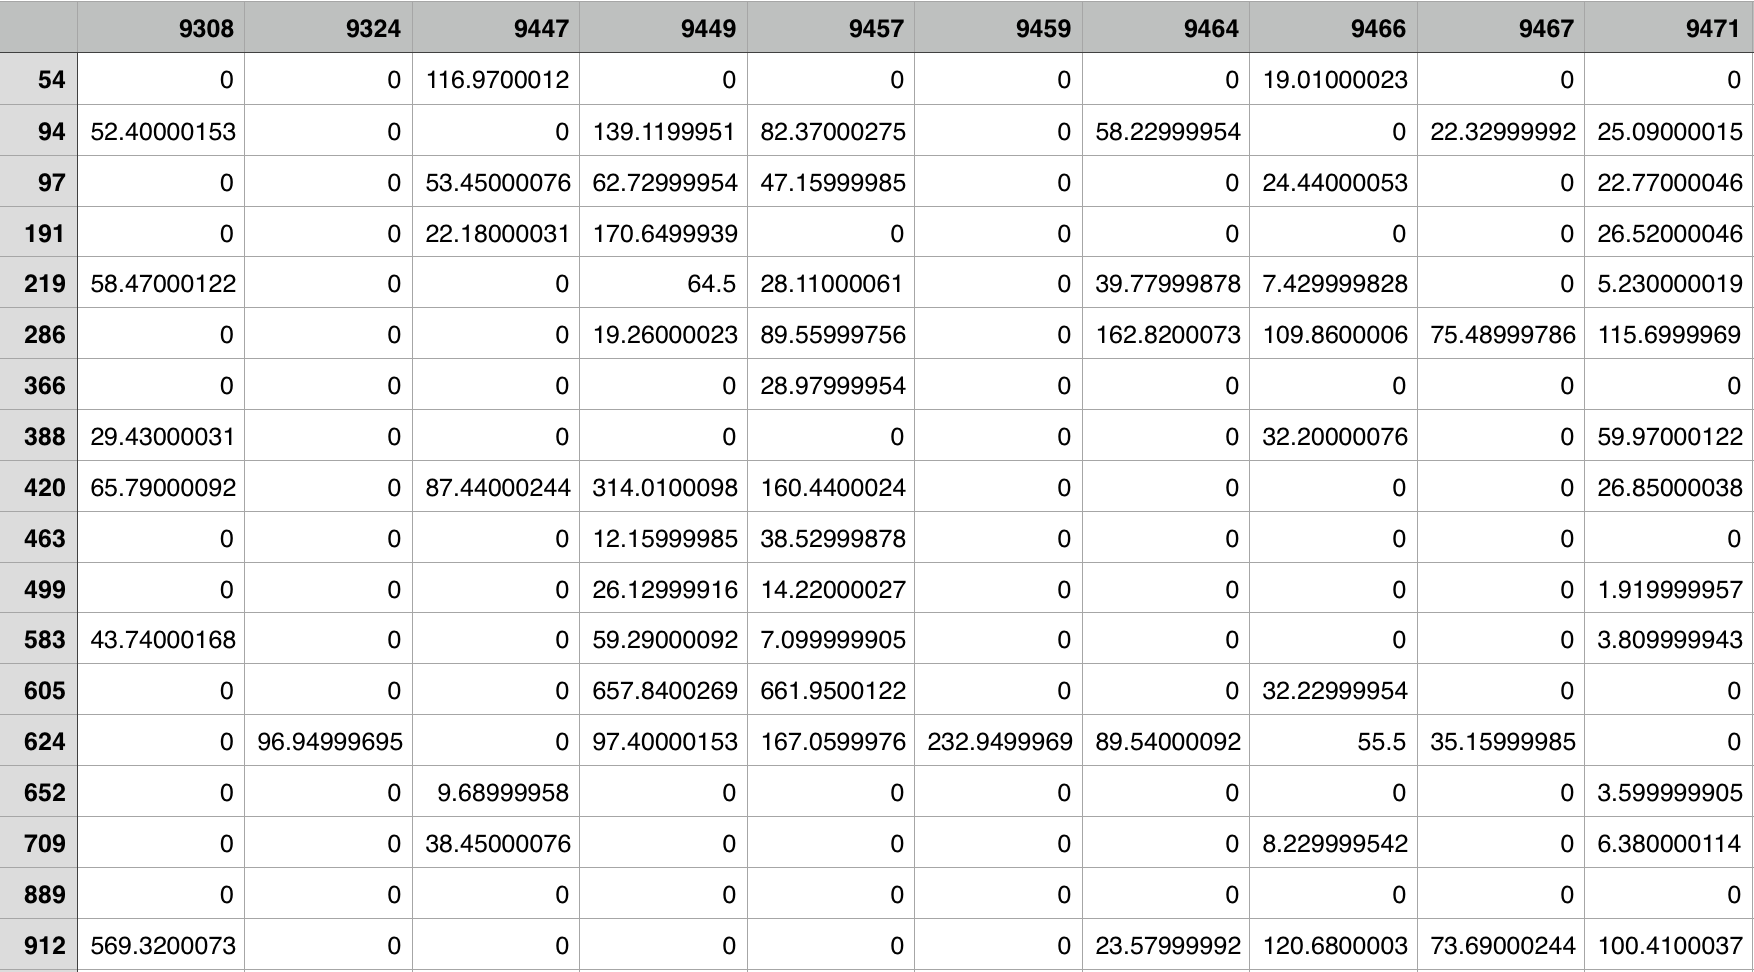
\includegraphics{feature.png}
  \caption{Example of 'feature.csv' pattern}
  \label{example feature}
\end{figure}
\begin{figure}[ht]
  \centering
  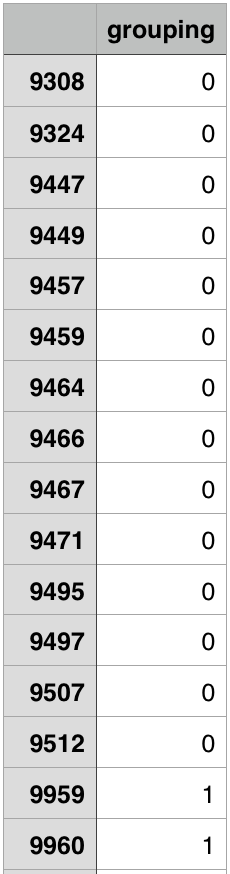
\includegraphics[width=2cm]{group.png}
  \caption{Example of 'group.csv' pattern}
  \label{example group}
\end{figure}


After creating the two csv.files, we need the paths for the two csv.files:

\begin{Schunk}
\begin{Sinput}
> path1 <- "/path/to/your/feature.csv/"
> path2 <- "/path/to/your/group.csv/"
\end{Sinput}
\end{Schunk}

Here for demonstration purposes, we use the data in the {\tt SDAMS} package

\begin{Schunk}
\begin{Sinput}
> directory1 <- system.file("extdata", package="SDAMS", mustWork=TRUE)
> path1<-paste(directory1,"ProstateFeature.csv",sep="/")
> directory2 <- system.file("extdata", package="SDAMS", mustWork=TRUE)
> path2<-paste(directory2,"ProstateGroup.csv",sep="/")
\end{Sinput}
\end{Schunk}

then use the function {\tt createSEsetFromCSV} after loading the {\tt SDAMS}
package.
\begin{Schunk}
\begin{Sinput}
> library("SDAMS")
> exampleSEset1 = createSEsetFromCSV(path1,path2)
> exampleSEset1
\end{Sinput}
\begin{Soutput}
class: SummarizedExperiment 
dim: 560 202 
metadata(0):
assays(1): counts
rownames(560): 93922 87209 ... 180624 130855
rowData names(0):
colnames(202): 9512 9963 ... 49341 49586
colData names(1): grouping
\end{Soutput}
\end{Schunk}

The feature data and grouping information can be accessed using
{\tt SummarizedExperiment} command:
\begin{Schunk}
\begin{Sinput}
> head(assay(exampleSEset1)[,1:10])
\end{Sinput}
\begin{Soutput}
        9512   9963  9965  9975   9979  9997 10015  10034  10044 10047
93922   0.00   0.00  0.00  0.00   0.00  0.00 68.97   0.00   0.00  0.00
87209   0.00   0.00  0.00  0.00   0.00  0.00  0.00   0.00   0.00 43.87
29633   0.00   0.00  0.00  0.00   0.00  0.00  0.00  57.21   0.00  0.00
40225   0.00 226.40  0.00 19.65   0.00  0.00  0.00   0.00   0.00  0.00
126342  0.00   0.00  0.00  0.00   0.00 20.43  0.00   0.00 109.93  0.00
42832  52.32 137.76 70.25  0.00 453.23 92.20  0.00 352.55 496.71  0.00
\end{Soutput}
\begin{Sinput}
> head(colData(exampleSEset1)$grouping)
\end{Sinput}
\begin{Soutput}
[1] 0 1 1 1 1 1
\end{Soutput}
\end{Schunk}


\subsection{Create SummarizedExperiment object from R global environment}
If the two datasets have been already claeaned and loaded into the R global
environment, we can use {\tt createSEsetFromEnvir} to create a
{\tt SummarizedExperiment} object.

\begin{Schunk}
\begin{Sinput}
> set.seed(100)
> featureInfo = matrix(runif(800,-2,5),ncol = 40)
> featureInfo[featureInfo<0] = 0
> rownames(featureInfo) = paste("feature",1:20,sep = '')
> colnames(featureInfo) = paste('subject',1:40,sep = '')
> groupInfo = data.frame(grouping=matrix(sample(0:1,40,replace = TRUE),ncol = 1))
> rownames(groupInfo)=colnames(featureInfo)
> exampleSEset2 = createSEsetFromEnvir(feature = featureInfo,group = groupInfo)
> exampleSEset2
\end{Sinput}
\begin{Soutput}
class: SummarizedExperiment 
dim: 20 40 
metadata(0):
assays(1): counts
rownames(20): feature1 feature2 ... feature19 feature20
rowData names(0):
colnames(40): subject1 subject2 ... subject39 subject40
colData names(1): grouping
\end{Soutput}
\begin{Sinput}
> head(assay(exampleSEset2)[,1:10])
\end{Sinput}
\begin{Soutput}
          subject1  subject2  subject3  subject4 subject5  subject6  subject7
feature1 0.1543628 1.7506781 0.3146237 1.2459082 1.216678 0.2919056 0.7766364
feature2 0.0000000 2.9756269 4.0558438 2.5297084 2.195787 0.7263509 0.7489158
feature3 1.8662570 1.7684409 3.4430911 4.7240116 4.438053 0.0000000 1.3078982
feature4 0.0000000 3.2428056 3.7911241 2.7347872 4.879769 0.5297764 2.0855984
feature5 1.2798450 0.9407102 2.2232705 1.1160362 0.000000 1.9968466 0.4667102
feature6 1.3863951 0.0000000 1.4386228 0.5044165 2.045562 2.7941617 0.0000000
         subject8 subject9  subject10
feature1 2.712745 3.705652 0.02105356
feature2 0.000000 1.978800 3.02481591
feature3 0.000000 1.360440 4.46378210
feature4 4.359349 0.000000 2.72457641
feature5 0.000000 0.000000 0.00000000
feature6 3.102040 0.000000 0.43647014
\end{Soutput}
\begin{Sinput}
> head(colData(exampleSEset2)$grouping)
\end{Sinput}
\begin{Soutput}
[1] 0 0 0 1 1 0
\end{Soutput}
\begin{Sinput}
> 
\end{Sinput}
\end{Schunk}

\section{Data Analysis}

Finally, we perform differential abundance analyais using
{\tt SummarizedExperiment} object created in the last section. This can be done
by using function {\tt SDA}. And a list with point estimates, p-values, q-values
and corresponding feature names is returned. Below is results generated by using
the {\tt SummarizedExperiment} object exampleSEset1.

\begin{Schunk}
\begin{Sinput}
> results = SDA(exampleSEset1)
> head(results$gamma)
\end{Sinput}
\begin{Soutput}
[1]  0.1100009  0.8629447 -0.7151261  0.2876821 -0.1251631  0.6292037
\end{Soutput}
\begin{Sinput}
> head(results$beta)
\end{Sinput}
\begin{Soutput}
[1] -0.04912170 -1.11354659 -1.30566809  0.02484749  0.53967121 -0.22075205
\end{Soutput}
\begin{Sinput}
> head(results$qv_gamma)
\end{Sinput}
\begin{Soutput}
[1] 0.4092097 0.1914385 0.2191259 0.3505466 0.3887992 0.1651784
\end{Soutput}
\begin{Sinput}
> head(results$qv_beta)
\end{Sinput}
\begin{Soutput}
[1] 0.7466379 0.2979437 0.2525717 0.7599717 0.2673415 0.3235222
\end{Soutput}
\begin{Sinput}
> head(results$qv_2part)
\end{Sinput}
\begin{Soutput}
          [,1]
[1,] 0.4622205
[2,] 0.1380966
[3,] 0.1192246
[4,] 0.4323376
[5,] 0.1806273
[6,] 0.1345612
\end{Soutput}
\begin{Sinput}
> head(results$feat.names)
\end{Sinput}
\begin{Soutput}
[1] "93922"  "29633"  "40225"  "126342" "42832"  "127351"
\end{Soutput}
\end{Schunk}



\section{Session Info}

\begin{Schunk}
\begin{Sinput}
> toLatex(sessionInfo())
\end{Sinput}
\begin{itemize}\raggedright
  \item R version 3.4.3 (2017-11-30), \verb|x86_64-apple-darwin15.6.0|
  \item Locale: \verb|en_US.UTF-8/en_US.UTF-8/en_US.UTF-8/C/en_US.UTF-8/en_US.UTF-8|
  \item Running under: \verb|macOS High Sierra 10.13.1|
  \item Matrix products: default
  \item BLAS: \verb|/Library/Frameworks/R.framework/Versions/3.4/Resources/lib/libRblas.0.dylib|
  \item LAPACK: \verb|/Library/Frameworks/R.framework/Versions/3.4/Resources/lib/libRlapack.dylib|
  \item Base packages: base, datasets, graphics, grDevices, methods,
    parallel, stats, stats4, utils
  \item Other packages: Biobase~2.36.2, BiocGenerics~0.22.1,
    DelayedArray~0.2.7, GenomeInfoDb~1.12.3, GenomicRanges~1.28.6,
    IRanges~2.10.5, matrixStats~0.53.1, S4Vectors~0.14.7, SDAMS~0.99.4,
    SummarizedExperiment~1.6.5
  \item Loaded via a namespace (and not attached): bitops~1.0-6,
    colorspace~1.3-2, compiler~3.4.3, GenomeInfoDbData~0.99.0,
    ggplot2~2.2.1, grid~3.4.3, gtable~0.2.0, lattice~0.20-35,
    lazyeval~0.2.0, magrittr~1.5, Matrix~1.2-12, munsell~0.4.3,
    plyr~1.8.4, qvalue~2.8.0, Rcpp~0.12.11, RCurl~1.95-4.10,
    reshape2~1.4.2, rlang~0.1.1, scales~0.4.1, splines~3.4.3,
    stringi~1.1.5, stringr~1.2.0, tibble~1.3.3, tools~3.4.3,
    trust~0.1-7, XVector~0.16.0, zlibbioc~1.22.0
\end{itemize}\end{Schunk}


\bibliography{reference}


\end{document}
